\chapter{Dynamic System Modeling}
\label{ch:sysModeling}

The goal of this section is to obtain a preliminary state-space model for the aeroservoelastic system in the form
\begin{align}
    \{\dot{x}\} &= [A] \{x\} + [B]\{u\} \\
    \{y\} &= [C] \{x\} + [D] \{u\}
\end{align}
based on first principles.

% +----------------------------------------------------------------------------+
% | EQUATIONS OF MOTION                                                        |
% +----------------------------------------------------------------------------+
\section{Equations of Motion}

The equations of motion for the general structural dynamic system with damping and forcing in the Laplace domain are
\begin{align}
    s^2 [M] \{q(s)\} + s [C] \{q(s)\} + [K] \{q(s)\} &= \{f(s)\}
\end{align}
where $\{q\}$ is the state expressed in the generalized modal coordinates, $\{f(s)\}$ is the generalized external forcing, and $[M]$, $[C]$, and $[K]$ are generalized mass, damping, and stiffness matrices respectively. Note that the modal coordinates include both elastic motions (of the structure) and rigid-body motions (of the structure and the control surfaces).
% The mass matrix, and stiffness matrix, and the mode shapes corresponding to $\{q\}$ are obtained from the NASTRAN model.

% The forcing for the aeroservoelastic wing can be decomposed into the aerodynamic forcing due to the state, the aerodynamic forcing due to gusts, and the forcing from actuator hinge moments:
% \begin{align}
%     s^2 [M] \{q(s)\} + s [C] \{q(s)\} + [K] \{q(s)\} &= q_D [A(s)] \{q(s)\} + q_D [A_G(s)] \frac{w_G}{U} + \begin{Bmatrix} \{0\} \\ \{H_c\} \end{Bmatrix}
% where $[A]$ is the aerodynamic influence matrix for the state, $[A_G]$ is the aerodynamic influence matrix for gusts, and ${H_c}$ is the hinge moment's influence.
The forcing for the aeroservoelastic wing can be decomposed into the aerodynamic forcing due to the state and the forcing from actuator hinge moments:
\begin{align}
    s^2 [M] \{q(s)\} + s [C] \{q(s)\} + [K] \{q(s)\} &= q_D [A(s)] \{q(s)\} + \begin{Bmatrix} \{0\} \\ \{H_c\} \end{Bmatrix}
\end{align}
where $[A(s)]$ is the aerodynamic influence matrix for the state and ${H_c}$ is the hinge moment's influence.

The whole system can be further decomposed into structural and control modes:
\begin{multline}
    \left( s^2 \begin{bmatrix}
        [M_{ss}] & [M_{sc}] \\
        [M_{cs}] & [M_{cc}]
    \end{bmatrix} + s \begin{bmatrix}
        [C_{ss}] & [C_{sc}] \\
        [C_{cs}] & [C_{cc}]
    \end{bmatrix} + \begin{bmatrix}
        [K_{ss}] & [K_{sc}] \\
        [K_{cs}] & [K_{cc}]
    \end{bmatrix} \right) \begin{Bmatrix}
        \{q_s(s)\} \\
        \{q_c(s)\}
    \end{Bmatrix} \\ = q_D \begin{bmatrix}
        [A_{ss}(s)] & [A_{sc}(s)] \\
        [A_{cs}(s)] & [A_{cc}(s)]
    \end{bmatrix} \begin{Bmatrix}
        \{q_s(s)\} \\
        \{q_c(s)\}
    \end{Bmatrix}
    % + q_D \begin{bmatrix}
    %     [A_{G,ss}(s)] & [A_{G,sc}(s)] \\
    %     [A_{G,cs}(s)] & [A_{G,cc}(s)]
    % \end{bmatrix} \frac{w_G}{U}
    + \begin{Bmatrix}
        \{0\} \\
        \{H_c\}
    \end{Bmatrix}
\end{multline}
The control modes are those corresponding to rigid-body motions of control surfaces. The structural modes are all other modes, including flexible-body modes and rigid-body modes of the entire model.

It is assumed that the dynamics of the control modes are completely determined by the control inputs and the inputs are not directly affected by the control modes, i.e. the actuators are irreversible controls. Then, interest is only in the dynamics of the structural modes:
\begin{multline}
    \left( s^2 \begin{bmatrix}
        [M_{ss}] & [M_{sc}]
    \end{bmatrix} + s \begin{bmatrix}
        [C_{ss}] & [C_{sc}]
    \end{bmatrix} + \begin{bmatrix}
        [K_{ss}] & [K_{sc}]
    \end{bmatrix} \right) \begin{Bmatrix}
        \{q_s(s)\} \\
        \{q_c(s)\}
    \end{Bmatrix} \\ = q_D \begin{bmatrix}
        [A_{ss}(s)] & [A_{sc}(s)]
    \end{bmatrix} \begin{Bmatrix}
        \{q_s(s)\} \\
        \{q_c(s)\}
    \end{Bmatrix}
    % + q_D \begin{bmatrix}
    %     [A_{G,ss}(s)] & [A_{G,sc}(s)]
    % \end{bmatrix} \frac{w_G}{U}
\end{multline}

Note that since the control modes are rigid-body modes, they have no stiffness ($[K_{cc}]$, $[K_{sc}]$, and $[K_{cs}]$ are zero) and the equations of motion further simplify to
\begin{multline}
    \left( s^2 \begin{bmatrix}
        [M_{ss}] & [M_{sc}]
    \end{bmatrix} + s \begin{bmatrix}
        [C_{ss}] & [C_{sc}]
    \end{bmatrix} + \begin{bmatrix}
        [K_{ss}] & [0]
    \end{bmatrix} \right) \begin{Bmatrix}
        \{q_s(s)\} \\
        \{q_c(s)\}
    \end{Bmatrix} \\ = q_D \begin{bmatrix}
        [A_{ss}(s)] & [A_{sc}(s)]
    \end{bmatrix} \begin{Bmatrix}
        \{q_s(s)\} \\
        \{q_c(s)\}
    \end{Bmatrix}
    % + q_D \begin{bmatrix}
    %     [A_{G,ss}(s)] & [A_{G,sc}(s)]
    % \end{bmatrix} \frac{w_G}{U}
\end{multline}

% +----------------------------------------------------------------------------+
% | THE ROGER APPROXIMATION                                                    |
% +----------------------------------------------------------------------------+
\section{The Roger Approximation}

% The aerodynamic influence matrices $[A]$ and $[A_G]$ are nonlinear functions of frequency. In order to obtain a linear state-space system, these must be approximated as analytic functions of $s$.
The aerodynamic influence matrix $[A]$ is a nonlinear function of reduced frequency $k$. In order to obtain a linear state-space system, it must be approximated as an analytic function of $k$.

The Roger approximation \cite{Roger1977} is a method of generating a rational function approximation of the aerodynamic influence matrix in the form
\begin{align}
    [A(jk)] &\approx [\bar{P}_0] + jk [\bar{P}_1] + (jk)^2 [\bar{P}_2] + \sum_{n=1}^{N_\text{lag}} \frac{jk}{jk+\bar{\beta}_n} [\bar{P}_{n+2}]
\end{align}
where $[P]$ are the unknown real-valued matrices that are fit to the tabulated matrices. Aside from the zeroth, first, and second order terms, there are $N_\text{lag}$ additional "lag term" approximating functions which are defined by their respective constants $\bar{\beta}$. The constants $\bar{\beta}$ are pre-determined

Given a tabulated set of known aerodynamic influence matrices across a range of reduced frequencies $k$,



For the $(1,1)$ element of an aerodynamic influence matrix $[A]$

% +----------------------------------------------------------------------------+
% | OUTPUT MODELING                                                            |
% +----------------------------------------------------------------------------+
\section{Output Modeling}


% +----------------------------------------------------------------------------+
% | ACTUATION AND SENSING DYNAMICS                                             |
% +----------------------------------------------------------------------------+
\section{Actuation and Sensing Dynamics}
When developing a model that is used for control design, the dynamics of the actuators and sensors must be accounted for. The output of the control law will be fed not into the plant, but the imperfect actuators. The input of the control law will come not directly from the plant, but from the imperfect sensors. The imperfect actuators and sensors can be accounted for in modeling by combining the actuator, plant, and sensor models into an integrated system model that can then be used for control design; see Fig. \ref{fig:actPlantSens} for a block diagram of this system of systems.
\begin{figure}[h]
    \centering
    \includegraphics[width=\textwidth]{ASEblockDiagram.png}
    \label{fig:actPlantSens}
    \caption{Integrated model of actuation, plant, and sensing in a control loop}
\end{figure}

The servo-actuated control surfaces on the wing and tail are known (from \cite{Quenzer2019}) to have dynamics according to the following transfer function\footnote{The numerator of this transfer function differs from that defined in \cite{Quenzer2019} because the actuator is calibrated to have unity DC gain before use.}:
\begin{align}
    G(s) &= \frac{1461}{s^2 + 62.2s + 1461}
\end{align}
This transfer function was then converted to the following equivalent state-space representation:
\begin{equation}
\begin{aligned}
    \label{eq:servoModel}
    s\{x\} &= \begin{bmatrix} -62.2 & -1461 \\ 1 & 0 \end{bmatrix} \{x\}
        + \begin{bmatrix} 0 \\ 1 \end{bmatrix} u \\
    y &= \begin{bmatrix} 0 & 1461 \end{bmatrix} \{x\}
\end{aligned}
\end{equation}
where $u$ is the input, $y$ is the output, and $\{x\}$ is the internal state of the actuator.

The wind tunnel gust vanes were measured to have no internal dynamics except for a pure time delay of 0.34 seconds. This pure delay was approximated as a second-order transfer function using a Pad\'e approximant:
\begin{align}
    G(s) &= \frac{s^2 - 176.47s + 10381}{s^2 + 176.47s + 10381}
\end{align}
The Pad\'e approximant matches the pure delay's response well in the frequency range of interest (<20 Hz); the step response and phase shift behavior of a pure delay and the Pad\'e approximant are compared in Fig. \ref{fig:padeApprox}.
\begin{figure}[H]
    \centering
    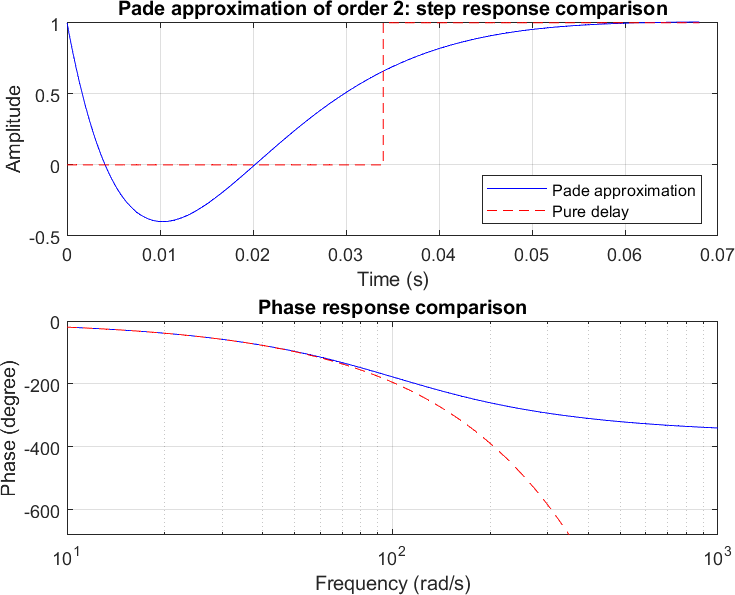
\includegraphics[width=4in]{padeApprox.png}
    \label{fig:padeApprox}
    \caption{Pad\'e approximant of the pure-delay response of the wind tunnel gust vanes}
\end{figure}
This transfer function was then converted to the following equivalent state-space representation:
\begin{equation}
\begin{aligned}
\label{eq:gustModel}
    s\{x\} &= \begin{bmatrix} -176.47 & -10381 \\ 1 & 0 \end{bmatrix} \{x\}
        + \begin{bmatrix} 1 \\ 0 \end{bmatrix} u \\
    y &= \begin{bmatrix} -352.94 & 0 \end{bmatrix} \{x\}
        + \begin{bmatrix} 1 \end{bmatrix} u
\end{aligned}
\end{equation}
where $u$ is the input, $y$ is the output, and $\{x\}$ is the internal state of the actuator.

The state-space models for the four actuators (three servo-actuated control surfaces and one pair of wind tunnel gust vanes) are combined to form one combined state-space model for all actuators with input, output, and state
\begin{align}
    \{u_\text{act}\} &= \begin{bmatrix} u_1 \\ u_2 \\ u_3 \\ u_4 \end{bmatrix} &
    \{y_\text{act}\} &= \begin{bmatrix} y_1 \\ y_2 \\ y_3 \\ y_4 \end{bmatrix} &
    \{x_\text{act}\} &= \begin{bmatrix} \{x\}_1 \\ \{x\}_2 \\ \{x\}_3 \\ \{x\}_4 \end{bmatrix}
\end{align}
respectively. The combined actuation state-space model is then
\begin{equation}
\begin{aligned}
    \{x_\text{act}\} &= \begin{bmatrix}
        [A_1] & & & \\ & [A_2] & & \\ & & [A_3] & \\ & & & [A_4]
        \end{bmatrix} \{x_\text{act}\}
        + \begin{bmatrix}
        [B_1] & & & \\ & [B_2] & & \\ & & [B_3] & \\ & & & [B_4]
        \end{bmatrix} \{u_\text{act}\} \\
    \{y_\text{act}\} &= \begin{bmatrix}
        [C_1] & & & \\ & [C_2] & & \\ & & [C_3] & \\ & & & [C_4]
        \end{bmatrix} \{x_\text{act}\}
        + \begin{bmatrix}
        [D_1] & & & \\ & [D_2] & & \\ & & [D_3] & \\ & & & [D_4]
        \end{bmatrix} \{u_\text{act}\}
\end{aligned}
\end{equation}
where the $[A]$, $[B]$, $[C]$, and $[D]$ system matrices for the two types of actuators are defined above in Eq. \ref{eq:servoModel} and \ref{eq:gustModel}. This then forms the actuator block shown in Fig. \ref{fig:actPlantSens}.

A similar process would be appropriate for a set of imperfect sensors. However, the high-rate sensors used in MARGE have approximately no dynamics in the frequency range of interest. Thus, the sensor response was approximated as
\begin{align}
    \{y_\text{sens}\} &= \{u_\text{sens}\}
\end{align}
In other words, the output of the sensor was taken as the output of the plant. This then forms the sensor block shown in Fig. \ref{fig:actPlantSens}.